\RequirePackage{nag}
\documentclass[12pt,letterpaper]{article}
\usepackage{lipsum}
% \usepackage{fixltx2e}
% \usepackage{classicthesis}
\usepackage{polyglossia}
\usepackage[natbib=true, 
			style=numeric, %authoryear or numeric; comp == compact
			bibstyle=nature, 
			backend=biber,
			uniquelist=false, 
			sorting=none,
			uniquename=false]{biblatex}
\usepackage{booktabs}
\usepackage{relsize}
\usepackage{setspace}
\usepackage{lineno}
\usepackage{wrapfig}
\usepackage{sidecap}

\setdefaultlanguage{english}
\setmainfont[Mapping=tex-text, 
			 Numbers=OldStyle, 
			 % SizeFeatures={{Size=12}}
			 ]{Times}
\setsansfont[Mapping=tex-text, 
			 Numbers=OldStyle, 
			 % SizeFeatures={{Size=12}}
			 ]{Helvetica}
\setmonofont[Scale=0.8]{Monaco}
\setcounter{secnumdepth}{0}

\addbibresource{ELI.bib}

% Set the line spread (height). Be careful here, use too small rather than too
% large value. Also: double-spaced lines correspond to a value of ~1.3,
% depending on the font, NOT to 2.0
\setstretch{1.1} % 1.1 normally

\graphicspath{{figs/}}

%% Custom macros

\newcommand*\captitle[1]{\textbf{#1}}
\newcommand*\todo[1]{%
    \graffito{\textcolor{red}{TO\ DO: #1}}}

\newcommand*\gene[1]{\textit{#1}}
\newcommand*\ko[1]{\textit{#1\textsuperscript{\(-/-\)}}}
\newcommand*\protein[1]{#1}
\newcommand*\species[1]{\textit{#1}}


\title{\ruleline{Logic Model}}
\lhead{Zhian N. Kamvar, Ph. D.}
\rhead{Logic Model}

\begin{document}
\maketitle
\begin{figure}[!htbp]
	\centering
	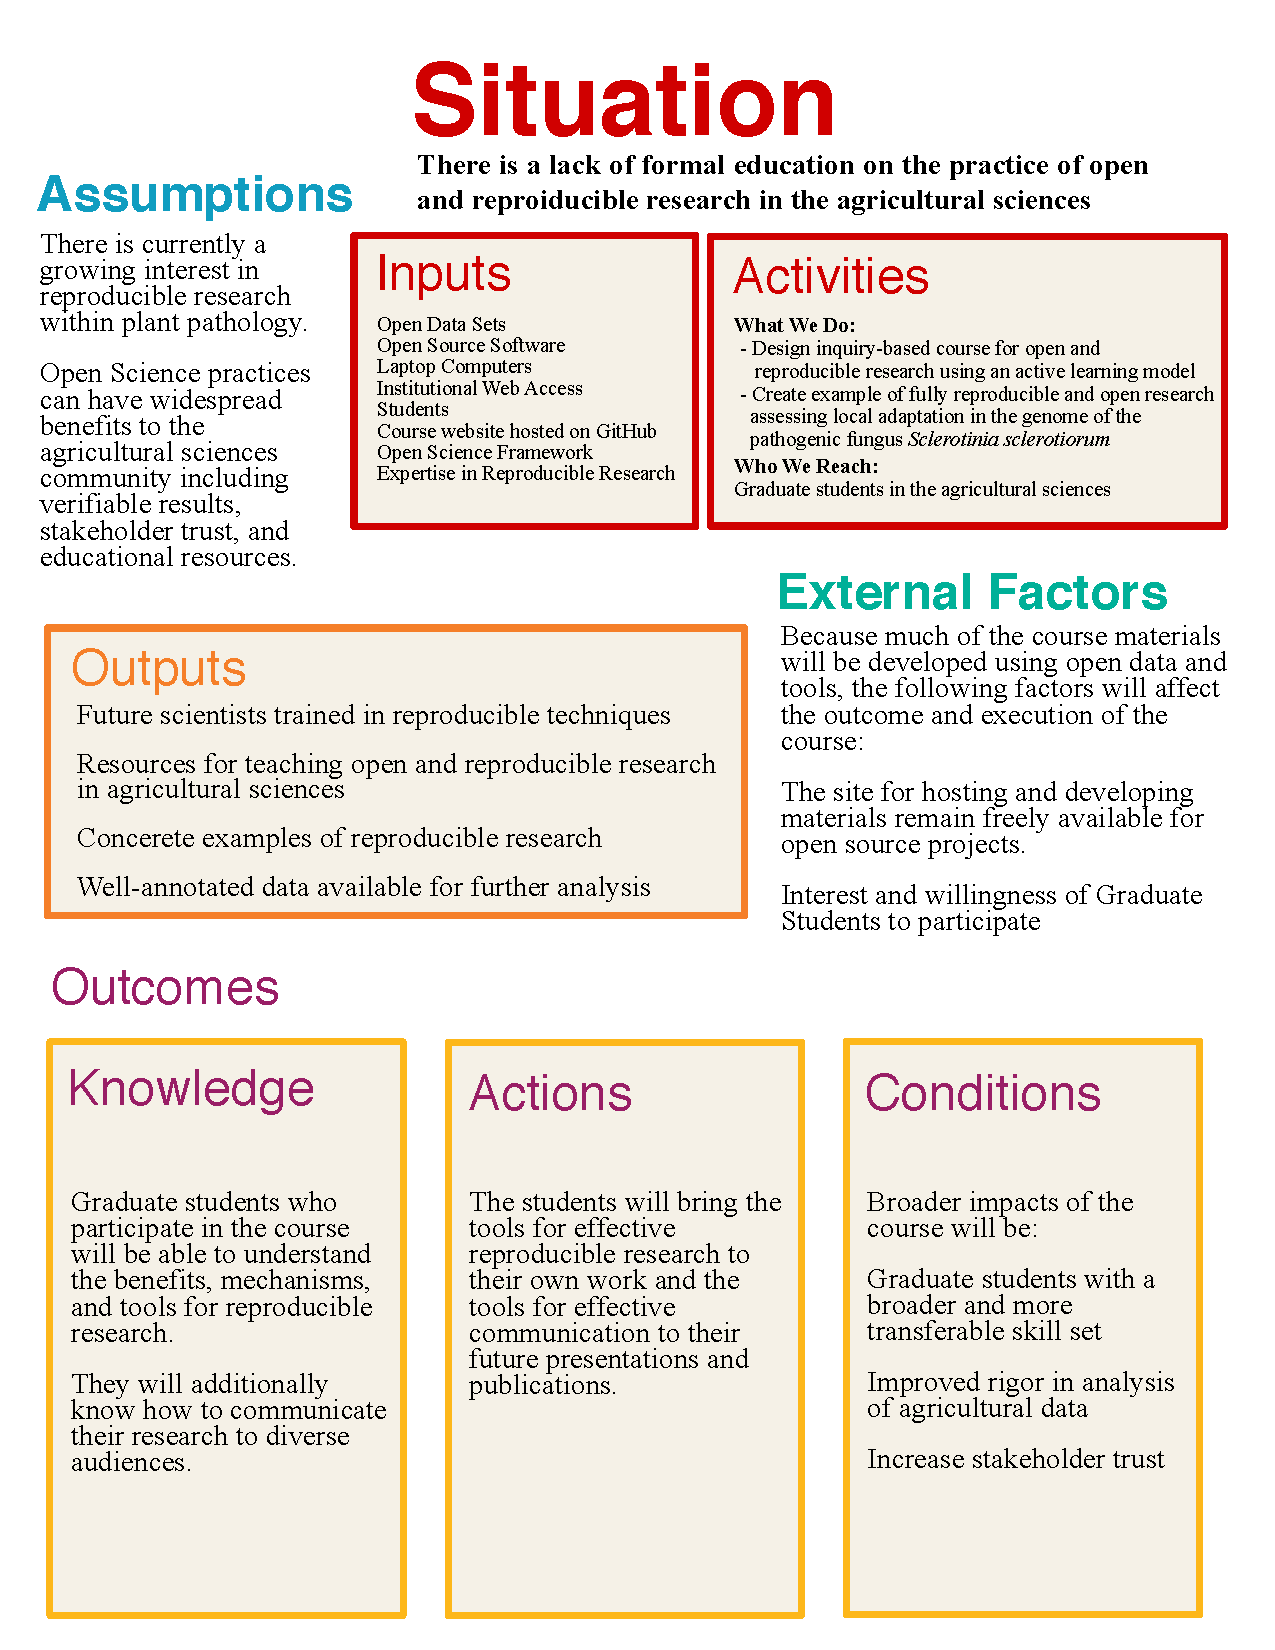
\includegraphics[width=\textwidth]{figure/logic-model.pdf}
\end{figure}



% % \textbf{2 page limit}

% % Include the elements of a logic model detailing the activities, outputs, and
% % outcomes of the proposed project. The logic model planning process is a tool
% % that should be used to develop your project before writing your application.
% % This information may be provided as a narrative or formatted into a logic model
% % chart. More information and resources related to the logic model planning
% % process are provided at \\
% % \url{https://nifa.usda.gov/resource/integrated-programs-logic-model-planning-process}.

% \section{Situation}

% % A description of the challenge or opportunity. The problem or issue to be
% % addressed, within a complex of socio-political, environmental, and economic
% % conditions.

% There is currently a lack of formal education on the practice of open and reproducible research.  

% % Education in agricultural data analysis needs a revitalization.
% % Current educational materials enforce best practices in experimental design and statistical theory, but fall short concerning data management, open science, and reproducible research.
% % Encouraging best practices in these areas have widespread benefits for the agricultural science community.
% % Open and well-managed data not only means that the results are easily verifiable, but that they can easily be built upon, and the data have a life outside of the original experiment.
% % These can have the effect of increased stakeholder trust, more opportunities for collaboration and funding, and a wealth of material for educators.

% % Many researchers are wary of sharing data, however.
% % Some fear they would not receive credit if these data are used by other researchers.
% % Others may not want to spend the time or energy to curate the data so that it is easily accessible. 
% % It is clear that there do not currently exist adequate incentives to data sharing. 

% % A solution to improving these practices in agricultural sciences may be to take an integrated approach where scientists share workflows associated with publications as cite-able education material. 
% % The American Phytopathological Society currently has an open on-line Education
% % Center (\url{http://www.apsnet.org/edcenter/Pages/default.aspx}), which hosts
% % peer-reviewed materials, but it has not seen any new material since 2014.
% % This resource could be used to host open data and dynamic workflows generated by plant pathologists, which would allow data to be open for educational use and reuse, providing all of the benefits of open science while removing many of the perceived drawbacks.


% \section{Inputs}

% % What is invested, such as resources, contributions, and investments that are
% % provided for the program.

% \begin{itemize}
% 	\item Open Data and Analyses
% 	\item Open Source Software
% 	\item Laptop Computers (personal or loaned)
% 	\item Institutional Web Access
% 	\item Students
% 	\item Classroom Space
% 	\item Course website hosted on GitHub (\url{https://github.com/})
% 	\item Open Science Framework (\url{https://osf.io/})
% 	\item Expertise in Reproducible Research
% \end{itemize}

% \section{Activities}

% % what the program does with its inputs to services it provides to fulfill its
% % mission.
% \subsubsection{What We Do:}

% \begin{itemize}
% 	\item Design inquiry-based course for open and reproducible research using an active learning model
% 	\item Design and execute example of fully reproducible and open research assessing local adaptation in the genome of the pathogenic fungus \textit{Sclerotinia sclerotiorum}
% 	\item Create special topics course at University of Nebraska-Lincoln
% 	\item Evaluate student performance based on understanding of the process of reproducible research
% \end{itemize}

% \subsubsection{Who We Reach:}

% \begin{itemize}
% 	\item Graduate students in the agricultural sciences
% \end{itemize}

% \section{Outputs}

% % Products, services and events that are intended to lead to the program's
% % outcomes.
% \begin{itemize}
% 	\item Future agricultural scientists trained to to reproducible research
% 	\item Resources for teaching open and reproducible research in agricultural sciences in the public domain
% 	\item Concrete examples of reproducible research in agriculture
% 	\item Well-annotated data available for further analysis
% \end{itemize}

% \section{Outcomes}

% % Planned results or changes for individuals, groups, communities, organizations
% % or systems.

% \subsection{Change in knowledge}

% % Occurs when there is a change in knowledge or the participants actually learn.
% Graduate students who participate in the course will be able to understand the benefits, mechanisms, and tools for reproducible research. They will additionally know how to communicate their research to diverse audiences.


% \subsection{Change in behavior}

% % Occurs when there is a change in behavior or the participants act upon what
% % they have learned.
% The students will bring the tools for effective reproducible research to their own work and the tools for effective communication to their future presentations and publications. 

% \subsection{Change in condition}

% % Occurs when a societal condition is improved.
% Broader impacts of the course will be

% \begin{itemize}
% 	\item Graduate students with a broader and more transferable skill set that results in
% 	\item Improved rigor in analysis of agricultural data which increases
% 	\item Stakeholder trust 
% \end{itemize}

% \section{External factors}

% % Variables that may have an effect on the portfolio, program, or project but
% % which cannot be changed by the managers of the portfolio, program, or project.

% Because much of the course material will be developed using open data and tools, the following factors will affect the outcome and execution of the course:

% \begin{itemize}
% 	\item GitHub continuing to be freely available for open source projects
% 	\item Interest and willingness of Graduate Students to participate
% \end{itemize}

% \section{Assumptions}

% % The premises based on theory, research, evaluation knowledge, etc. that
% % support the relationships of the elements of the logic model and upon which
% % the success of the portfolio, program, or project rests.
% The creation of this course and materials are based on the assumptions that
% \begin{itemize}
% 	\item There is currently a growing interest in reproducible research within plant pathology.
% 	\item Open science practices can have widespread benefits to the agricultural sciences community including easily verifiable results, stakeholder trust, and a plethora of resources for the development of educational materials. 
% \end{itemize}





\end{document}
